\begin{figure*}[!htbp]
\begin{center}

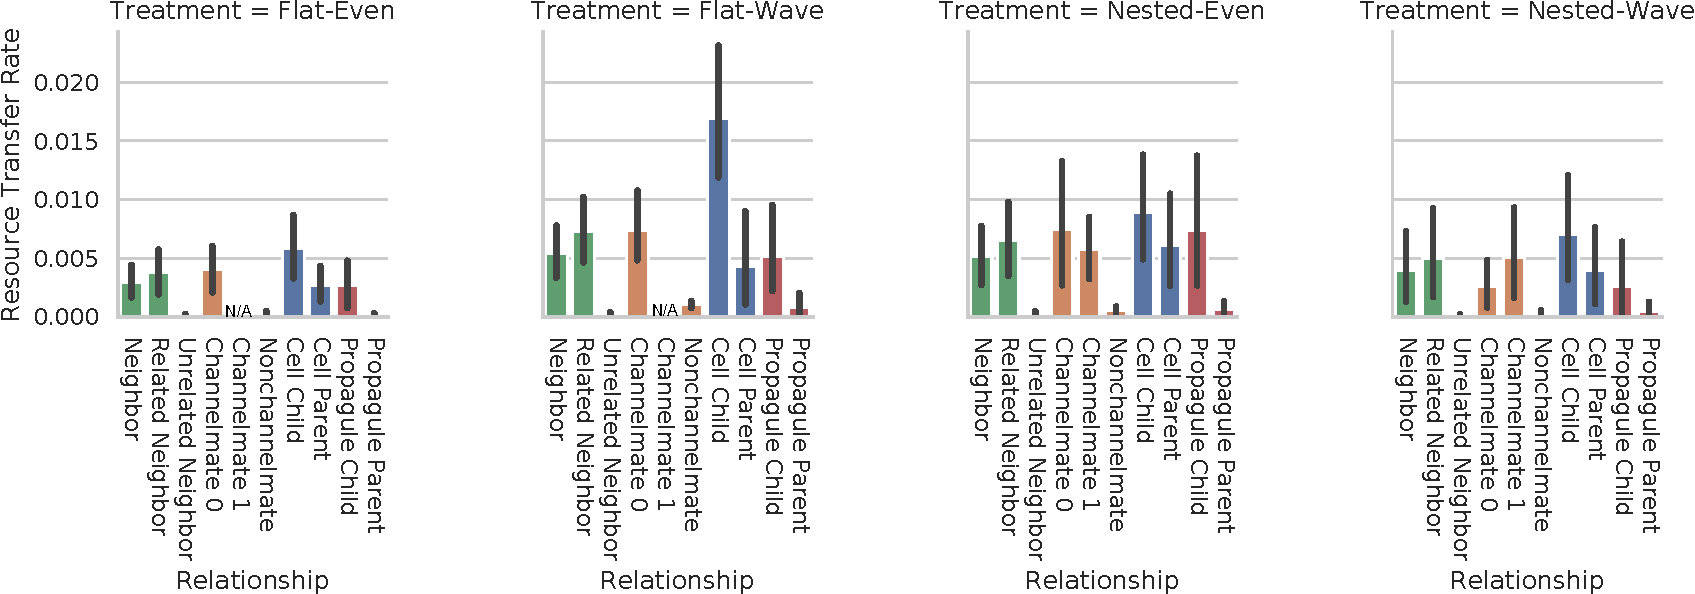
\includegraphics[width=\textwidth]{sharing/title=Resource_Transfer_Rate+_data_hathash_hash=ade957ec08284082+_script_fullcat_hash=ed8603f4ffa9a1af+_source_hash=53a2252-clean+ext=}

\caption{
Resource sharing rates across donor-recipient relationships.
Neighbor describes any potential recipient cell.
Related neighbor describes a recipient cell that is a direct cellular progenitor or offspring of the donor, registered to a same signaling channel as the donor, or a member of a signaling channel that is a progenitor or offspring of the donor's.
Unrelated neighbors constitutes all neighbors that are not related neighbors.
Channelmate refers to donor-recipient pairs that are registered to a same signaling channel.
Note that level-one groups are not defined in the flat treatment.
Non-channelmate recipients are not registered to any same signaling channel in common with the potential donor.
Cell child and parent describe direct nuclear cell relationships between donor and recipient.
Finally, a propagule child relationship exists when a donor cell is a member of the highest-level signaling channel that directly begat the recipient's.
A propagule parent relationship describes the converse.
Error bars indicate 95\% confidence.
}
\label{fig:sharing}
\end{center}
\end{figure*}
